\documentclass[12pt,letterpaper]{article}

% just for the example
\usepackage{lipsum}
% Set margins to 1.5in
\usepackage[margin=1.5in]{geometry}
\usepackage[toc,page]{appendix}

% for graphics
\usepackage{graphicx}
\graphicspath{{./figures/m3/}}

% for crimson text
\usepackage{crimson}
\usepackage[T1]{fontenc}
\usepackage{url}

% setup parameter indentation
\setlength{\parindent}{0pt}
\setlength{\parskip}{6pt}

% for 1.15 spacing between text
\renewcommand{\baselinestretch}{1.15}

% For defining spacing between headers
\usepackage{titlesec}
% Level 1
\titleformat{\section}
  {\normalfont\fontsize{18}{0}\bfseries}{\thesection}{1em}{}
% Level 2
\titleformat{\subsection}
  {\normalfont\fontsize{14}{0}\bfseries}{\thesection}{1em}{}
% Level 3
\titleformat{\subsubsection}
  {\normalfont\fontsize{12}{0}\bfseries}{\thesection}{1em}{}
% Level 4
\titleformat{\paragraph}
  {\normalfont\fontsize{12}{0}\bfseries\itshape}{\theparagraph}{1em}{}
% Level 5
\titleformat{\subparagraph}
  {\normalfont\fontsize{12}{0}\itshape}{\theparagraph}{1em}{}
% Level 6
\makeatletter
\newcounter{subsubparagraph}[subparagraph]
\renewcommand\thesubsubparagraph{%
  \thesubparagraph.\@arabic\c@subsubparagraph}
\newcommand\subsubparagraph{%
  \@startsection{subsubparagraph}    % counter
    {6}                              % level
    {\parindent}                     % indent
    {12pt} % beforeskip
    {6pt}                           % afterskip
    {\normalfont\fontsize{12}{0}}}
\newcommand\l@subsubparagraph{\@dottedtocline{6}{10em}{5em}}
\newcommand{\subsubparagraphmark}[1]{}
\makeatother
\titlespacing*{\section}{0pt}{12pt}{6pt}
\titlespacing*{\subsection}{0pt}{12pt}{6pt}
\titlespacing*{\subsubsection}{0pt}{12pt}{6pt}
\titlespacing*{\paragraph}{0pt}{12pt}{6pt}
\titlespacing*{\subparagraph}{0pt}{12pt}{6pt}
\titlespacing*{\subsubparagraph}{0pt}{12pt}{6pt}

% Set caption to correct size and location
\usepackage[tableposition=top, figureposition=bottom, font=footnotesize, labelfont=bf]{caption}

% set page number location
\usepackage{fancyhdr}
\fancyhf{} % clear all header and footers
\renewcommand{\headrulewidth}{0pt} % remove the header rule
\rhead{\thepage}
\pagestyle{fancy}

% Overwrite Title
\makeatletter
\renewcommand{\maketitle}{\bgroup
   \begin{center}
   \textbf{{\fontsize{18pt}{20}\selectfont \@title}}\\
   \vspace{10pt}
   {\fontsize{12pt}{0}\selectfont \@author} 
   \end{center}
}
\makeatother

% Used for Tables and Figures
\usepackage{float}

% For using lists
\usepackage{enumitem}

% For using APA Citation format
\usepackage{apacite}

% Custom Quote
\newenvironment{myquote}[1]%
  {\list{}{\leftmargin=#1\rightmargin=#1}\item[]}%
  {\endlist}
  
% Create Abstract 
\renewenvironment{abstract}
{\vspace*{-.5in}\fontsize{12pt}{12}\begin{myquote}{.5in}
\noindent \par{\bfseries \abstractname.}}
{\medskip\noindent
\end{myquote}
}

\begin{document}

% Set Title, Author, and email
\title{Assignment M4}
\author{Snejana Shegheva \\ sshegheva3@gatech.edu}

\maketitle
\thispagestyle{fancy}

\begin{abstract}
Mapping data from one form to another for its ease-of-use is at the core of the \textit{Extract, Transform and Load} process. In this project, we evaluate various prototypes for an internal interface of a \textit{transform} task that prepares the data for use in a personalized recommendation system powered by Artificial Intelligence engines. The task involves altering the form of the received data with a purpose to extract relevant features in the form that is more advantageous for subsequent tasks. Our main goal is to assess all the weak areas of the suggested alternative models via early feedback collection from users who perform the task frequently and therefore have a good understanding of the task at hand.  
\end{abstract}

\section*{Qualitative Evaluation}
\subsubsection*{Think-aloud for Verbal Prototype}
\textit{Appendix} B contain verbal prototype that discusses a possible interface where a user is given a recommendation for which transformation function(s) is most compatible with the observed variable. The interface target novices who need to explore the system, and experts who aim to perform their tasks more efficiently.

\textbf{Evaluation Plan}
For this stage of evaluation, the plan is to engage a single user in the think-aloud study. The chosen user, Product Manager with a client-facing role, has significant experience with the task at hand and is expected to provide good feedback on the prototype that is delivered verbally. The evaluation will take place in the work setting where the user will be suggested an alternative way to perform their usual task of data transformation. The results of the conversation will be summarized and recorded \textit{after} the exchange takes place. Any notes drafted during the discussion will be collected as artifacts of the study. The goal of this evaluation is to collect early feedback on the suggested idea and estimate user's interest in taking it to the next step of implementation.

\textbf{Think-Aloud Study}
To get started with the evaluation of the verbal prototype, I will, first, describe the idea to the user so they can imagine their workflow within the new interface. After they confirm the understanding of new direction, I will ask them to perform a specific transformation task while thinking aloud through the steps. My directions will be based on actual use cases, and allow freedom in the execution of the task, i.e., I will not be providing detailed instructions on \textit{how} to accomplish the goal.

\textit{Question 1 - Use case}: Let's say you have collected data on the recently published papers in the field in Machine Learning and Artificial Intelligence. You have a field that contains a list of \textit{keywords}, and let's assume you only want to get the first-mentioned keyword from the list. How would you accomplish this task in the new interface?  

\textit{Question 2 - Use case}: Let's say that in the same data set, you have a field that captures the \textit{published date}. If you would like to split this into a \textit{year} and \textit{month} variable, how would you go about it?

\textit{Question 3 - Use case}: Let's say you have two \textit{date} fields - \textit{submission date} and \textit{acceptance date}. Your goal is to create a variable that stores the elapsed time between the two dates. Do you think the new interface will sufficiently guide you through the process? What do you imagine the interface should do if you are stuck on the task, such as - the recommendations for the transformations do not capture your intentions very well?   

\textit{Question 4 - General Satisfiability}: What tasks in your opinion are more efficiently performed in the new interface when compared to the current version? How about less efficiently? Would you still prefer the current interface and why? 

\textit{Question 5 - Learnability}: Do you expect a significant amount of guidance from the interface, and which areas? For example, would you be able to find the variables you need to change quickly? How quickly do you expect to see a transformation that suits your needs? Do you plan to request a different set of recommendations? Would you like to quickly access \textit{all} available transformations? 

\textbf{Meeting the Requirements} \textit{Appendix A} lists the requirements identified at the earlier stages of the need-finding phase. The evaluation plan covers all three areas of the requirements - functionality, usability, and learnability. By analyzing the results of the think-aloud study, I hope to further narrow down into the \textit{data inventory} on \textbf{what are the user's goals, tasks, and subtasks?} and \textbf{what are their needs?}.  Successfully executing the plan will result in a data that would give insights into efficiency, learnability, and satisfaction of the new interface when compared to the currently used interface. The crucial metric of this evaluation plan is to assess whether or not the user's needs have been met. A detailed list of \textit{hits} and \textit{misses}, in addition to the user's overall sentiment will serve as a decision rule on whether or not to advance the suggested prototype to the next stage. 


\section*{Empirical Evaluation\footnote{This section of the assignment is based on the lecture notes and Chapter 5 from the \cite{mackenzie2012human} book}}
\textit{Appendix C}  contain as a candidate for the Textual prototype: Start with a list of most common transformations, and map them to one or more data variables. The interface target experts who aim to perform their tasks more efficiently by quickly searching through the transformations and applying them in bulk operation.

\textbf{Control and Experimental Conditions}
The goal of the empirical evaluation for the task described in the prototype is to \textit{compare} the efficiency of the task in the current and the new interface. We design three experiments that asks the users to complete same tasks in two different settings: \textit{control} - current interface, and \textit{treatment} - new prototype interface. The experiments intend to analyze the relationship between two variables - dependent and independent - to answer testable questions:  whether or not the new interface is advantageous to the current interface.

\hspace{10mm} \textbf{Independent variable}: Interface - \textit{Current} or \textit{New}  

\hspace{10mm} \textbf{Dependent variables}: 


\hspace{20mm} - Average number of steps across three different tasks 


\hspace{20mm} - Average task completion time across three different tasks

To run an experiment that decides which interface is superior regarding the speed and efficiency, we design three tasks that cover most of the everyday use cases ranging from simple to more advanced. 

\textbf{Task 1} Splitting one variable in two separate variables
\begin{itemize}
    \item Initial step (not measured): Load data with a field that contains \textit{Full Names}. 
    \item Create a new variable that contains only the first name
    \item Create a new variable that contains only the last name
\end{itemize}

\textbf{Task 2} Combining two variable into one by using a mathematical function
\begin{itemize}
    \item Initial step (not measured): Load data with a field that contains \textit{start} and \textit{end date}. 
    \item Create a new variable that computes the number of days between the start and the end
\end{itemize}

\textbf{Task 3} Chain multiple transformations by using the output of the previous as an input to the next one
\begin{itemize}
    \item Initial step (not measured): Load data with a field that contains unstructured text. 
    \item Create a new variable that cleans the text variable by correcting typos.
    \item Create a new variable extract keywords from the \textit{corrected} text
    \item Create a new variable that assigns the keywords a category
\end{itemize}


\textbf{Null Hypothesis}. Both interfaces provide the \textit{same} efficiency for accomplishing all three tasks (i.e., there is no difference in the final outcomes)

\textbf{Alternative Hypothesis}. Accomplishing the three tasks is \textit{faster} using the new interface as measured by average completion time and number of steps required to perform given tasks (i.e., the new interface is superior)

\bigskip
Since the number of participants is very small, and their experience with the task may vary (therefore significantly skewing the results), it makes sense to use \textit{within-subjects} method, in which the same user is asked to perform given tasks with the current and with the new interface. The three tasks described above will \underline{collect two data points}: number of steps taken, and total time to complete a task. Since the dependent variable is expressed with \textit{ratio} data, we are going to analyze the results with \textbf{Student's t-test}, or, alternatively, with MWW or Kruskal-Wallis test. 

In the experiments for interface efficiency, we are going to \textbf{control} for variables such as \textit{time of the day} and \textit{weekday vs. weekend} to reduce the effect they may have on the measured outcomes. It may take it less time for users to execute the tasks early in the morning vs. at the end of the day when their cognitive resources are more depleted. 

Finally, two circumstances may change systematically between the experiments that might cause the results to be misinterpreted. One \textbf{confounding} variable is \textit{previous user experience} with the existing interface. If the total time to complete the tasks is significantly lower in the existing interface vs. the new prototype, then the effect of \textit{familiarity}  confounded the experiments. In this case, focusing on the number of steps instead of time can help reduce the impact.

Another variable with a similar effect is due to the experiment setup. The order of the treatments matters because it provides the user with an opportunity to re-use knowledge between experiments. As we are presenting the same tasks in both trials, with the same participants, the time it takes to solve the task the second time may be only incremental nature. For example, when repeating the task in the different interface, the participant had already solved for what type of a transformation function is most applicable to the task. This effect could be potentially controlled for by varying the task's details slightly without changing its difficulty level.


\section*{Predictive Evaluation}

We are going to perform a \textbf{Cognitive Walkthrough} on the prototype shown in \textit{Appendix D}. The wireframes guide the user through the transformation task by keeping the sample of the data visible at all times. 

For the Cognitive Walkthrough, we need to identify the sequence of actions along with the series of questions that helps us evaluate the prototype.

\begin{itemize}
    \item \textbf{Step 1}: Select the variable to transform
    \begin{itemize}
        \item Does the user understand what does it mean for a variable to be selected?
        \item Can the user see how the selection is accomplished? Is it visible on the screen or it requires filtering and contextual menus?
        \item Is the source variable clearly labeled?
        \item If the user is unable to select a variable, and the feedback is given to the user, can they understand and apply the feedback? 
    \end{itemize}
    \item \textbf{Step 2}: Apply the desired transformation function
    \begin{itemize}
        \item Does the user have a correct conceptual model for that it means to change/transform the variable?
        \item Can the user see the list of available transformation functions?
        \item Do the functions' names reflect the clear operation? 
        \item If the user selects an incompatible transformation, is the feedback given to the user helpful and sufficient to correct their actions?
    \end{itemize}
    \item \textbf{Step 3}: Confirm the result for the transformation
    \begin{itemize}
        \item Does the user grasp how to evaluate the effect of the applied transformation?
        \item Can the user see what type of transformation function has been applied to the variable?
        \item Can the user infer if the transformation has been propagated (applied) or just saved (configured) on the screen?
        \item Can the user infer based on the feedback if the transformation is successful or not?
    \end{itemize}
\end{itemize}

The users will be accomplishing the sequence of steps described above in the context of the new interface. Although they would be experienced in the task of transformation, they would have to navigate in an unfamiliar interface and discover the methods required to complete the tasks. The questions defined in each sub-task can be used to evaluate the prototype and compare its usability between users with varying degree of experience on the task. 

The success of the prototype will be measured by the number of affirmative answers to the questions. For any item that has been answered as "NO," we will supply an explanation and a recommendation to resolve the gap. For example, if the user cannot find the functionality they look for because it is incorrectly labeled or not visible on the screen, the outcome of this evaluation will augment the prototype with additional features to complete the requirements. 

A limitation of the predictive evaluation is that for some of the steps we cannot get the affirmative answers because the interface does not exist yet. We cannot predict if the user would understand the feedback because then we do not show the actual feedback in the prototype. We might provide examples of possible feedback, and how and where it would be revealed, but we will not be able to anticipate the user's response. 

\section*{Preparing to Execute}

Without an actual interface, it will not be possible for us to carry out the Empirical Evaluation, mainly because it collects the quantitative data such as time elapsed between the start and the end of the task, and the number of steps taken to complete the task. Therefore, we postpone this evaluation plan for future iterations. 

The Qualitative Evaluation is typically performed in the early stages of prototyping. The feedback from users can inform the subsequent iterations of needfinding and prototyping. At this stage, it is essential to evaluate if the users' needs have been sufficiently met before proceeding to implementations that can be more costly regarding time and allocated resources. 

Since the Prediction Evaluation does not involve users, it is very \textit{cheap} and relatively efficient for informing ongoing design decisions, such as the positions and labeling of functionality required for accomplishing the task. This evaluation plan helps us formalize the user's thought process through the analysis of well-defined methods and operators. 

In conclusion, we choose to \textit{advance} the Qualitative and Predictive Evaluations, and \textit{drop} the Empirical Evaluation.  

\bibliographystyle{apacite} 
\bibliography{bibtemp}

\newpage
\section*{Appendices}

\appendix


\subsection*{A}
\subsection*{Requirements}

\textbf{Functionality} - range of tasks supported for data transformation.

1) The interface must let user \textit{select} a source data intended for modification, \textit{choose} a transformation, \textit{save} the configuration and \textit{apply} the task to the dataset.

2) The interface should give the user a preview of the outcome for selected transformation \textit{before} the task is applied.

3) The interface should allow the user to create/edit/delete transformations, and optionally export it to a human-readable form.

\textbf{Usability} - quality of the available functionality.

1) The interface must support a transformation that is based on multiple sources, for example, combining two fields into one, or performing mathematical operations on them.

2) The interface must provide clear distinction between actions for \textit{saving} a configuration for a transformation, or \textit{applying} the transformation the data.

\textbf{Learnability} - ease and speed for the task of transforming data.

1) The interface should have a toolbox of standard transformations with meaningful names, and built-in tooltip that expands the capabilities of each transformation with examples.

2) The interface should provide clear messaging and notifications on the system's progress. For example, what is the most recent user's request, and what is its status.

3) The interface should allow the user to change the preferences on the order of the available transformations. The current order is alphabetical, and it does not help locate the needed transformation quickly. Options for ordering may include: 

\begin{itemize}
    \item Sort by relevance. Can the interface autodetect the transformations most compatible with the selected data type?
    \item Sort by recency. Show the transformations on top which were accessed last.
    \item Sort by popularity. A user may have a subset of transformations they access the most frequently so it may be convenient to show a different set of transformations on top without requiring the user to scroll through the large list. 
\end{itemize}


\subsection*{B}

\subsection*{Prototype 1 - Verbal}

\textit{Imagine that you have an interface through which you can interact with the incoming streams of data. Your goal is to apply some rules to the received data dynamically. Those rules would transform the current and future data into the desired alternative output. You can treat these transformation rules as simple mathematical functions.}

\textit{The way the system currently works is by iterating through all variables, one at a time, giving the user an option to edit variable. To find a rule, you need to parse through a pile of currently available transformations to find the one most relevant to you. This, of course, could be a daunting task if transformations are not organized in any meaningful way.}

\textit{Imagine an alternative way of interacting with a system like that. Let's take as an example a case where you might be looking at a variable that contains a large chunk of text (maybe, transcripts from video lectures). The interface could recommend you a list of most likely transformations, such as:
\begin{itemize}
    \item Remove all punctuation (which could be useful for some subsequent NLP tasks)
    \item Extract keywords (instead of passing the entire text through the pipeline, you might be only interested in the topmost representative terms, and entities) 
\end{itemize}
}

\textit{The set you are given back is limited to the selected data type. For example, it won't recommend you transformations intended for numerical fields, such as Averaging, Adding/Subtracting, Computing rates, etc. This way your task of transforming can be optimized to your data leading to a more efficient workflow. What do you think?}

\subsection*{C}

\subsection*{Prototype 2 - Textual}

\textbf{The Idea}.
Users are presented with a list of Transformations that allows them to apply the same rule to a set of fields in a \textit{single} instruction (think one-to-many as opposed to one-to-one described in the previous prototype)

\textbf{How it Works}. In order to perform any transformations on the input data, a user A) navigates to a dedicated Tab that lists transformation organized in alphabetical order by default; B) The user selects a transformation and is subsequently presented with the set of all available fields compatible with the chosen transformation; C) User highlights the areas they wish to apply the transformation to, and hits Save. Then repeat the process if other transformations are needed.

\textbf{Example}. \textit{User decides to clean the unstructured data by removing all special characters and maybe stop words as well. Users find a transformation "Remove Punctuation," and observes that half of the available fields for transformations become disabled (greyed out) since they represented numerical data or date ranges. From the subset of variables, the user selects data fields - "summary," "keywords," and "content" - and applies the selected transformation. Then user finds another transformation "Remove STOP words," and repeats that for the fields "summary."}

\subsubsection*{Functionality}

\begin{itemize}
    \item The page with the transformation \textbf{displays the top 10 choices} and provides a pagination mechanism in addition to a customization for how many results are shown on the page.
    \item The transformations are \textbf{searchable} by the names and their descriptions. 
    \item The transformations are \textbf{sortable} by relevance, recency, popularity, date of creation and date of update.
    \item Data fields available for a select transformation are \textbf{dynamic}. Incompatible fields are greyed out leaving user with a more manageable set.
    \item User is given an option to \textit{apply}, \textit{save}, and \textit{export} the current configuration in JSON format.
\end{itemize}

\subsection*{D}
\subsection*{Prototype 3 - Wireframes}
The task described in this project involves knowledge of data intended for transformations. Providing the user with a view that shows a sample of the data aligns well with the \textit{perceptability} principle that keeps the user informed about what is going on through appropriate feedback \cite{nielsen1994usability}. Figure~\ref{fig::2} start with a view of the data (similar to a DataFrame concept in pandas \cite{mckinney2011pandas})

\begin{figure}[h]
\centering
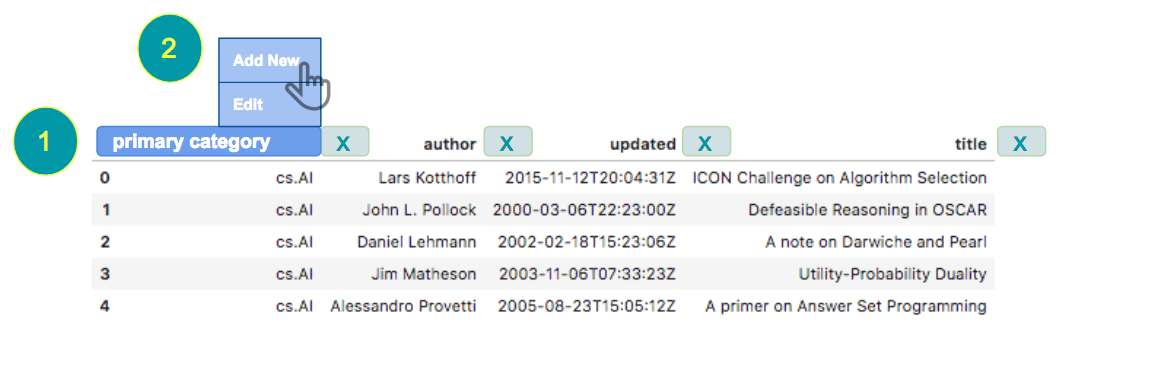
\includegraphics[scale=.3]{figures/m3/wireframe-screen1.png}
\caption{Screen 1: User selects a variable and is given a choice to either edit the existing variable or create a new one based on the selected. Data is retrieved via https://arxiv.org/'s API}
\label{fig::2}
\end{figure}

The user workflow can be described by: 

\begin{itemize}
    \item Select a variable that intended for a transformation. The variable name is highlighted (see Figure~\ref{fig::2}, step 1)
    \item A context menu appears that gives user an option to either \textit{Edit} the existing variable, or \textit{Add New}  (see Figure~\ref{fig::2}, step 2)
    \item Upon selecting to Add a new Variable based on the highlighted field, the user is given a list of Transformations to choose from (See Figure~\ref{fig::3})
    
\begin{figure}[h]
\centering
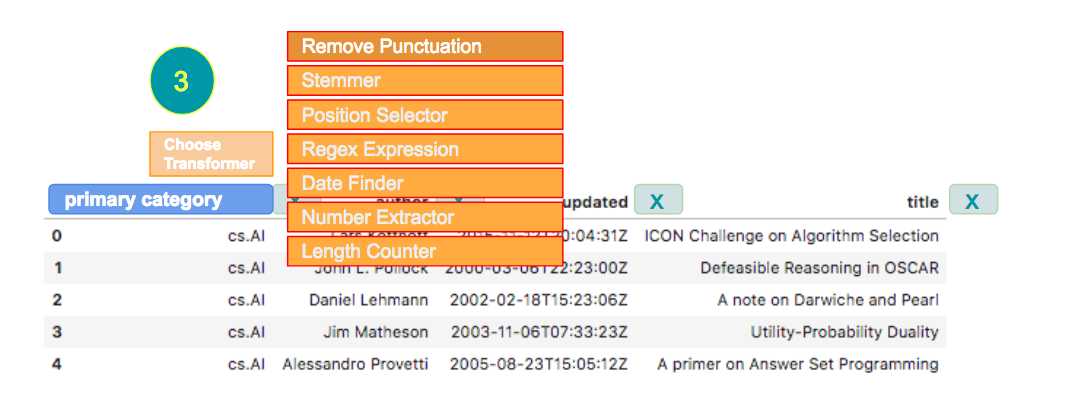
\includegraphics[scale=.3]{figures/m3/wireframe-screen2.png}
\caption{Screen 2: User is given a list of transformations to choose from}
\label{fig::3}
\end{figure}

    \item After the user selected a transformation, a \underline{new block} is created with \underline{a link} to the original variable. A user is prompted to give the new variable a name (see Figure~\ref{fig::4}). The \textit{attached} transformation is kept in the block to remind the user on the selected transformation rule. 
    
    
\begin{figure}[h]
\centering
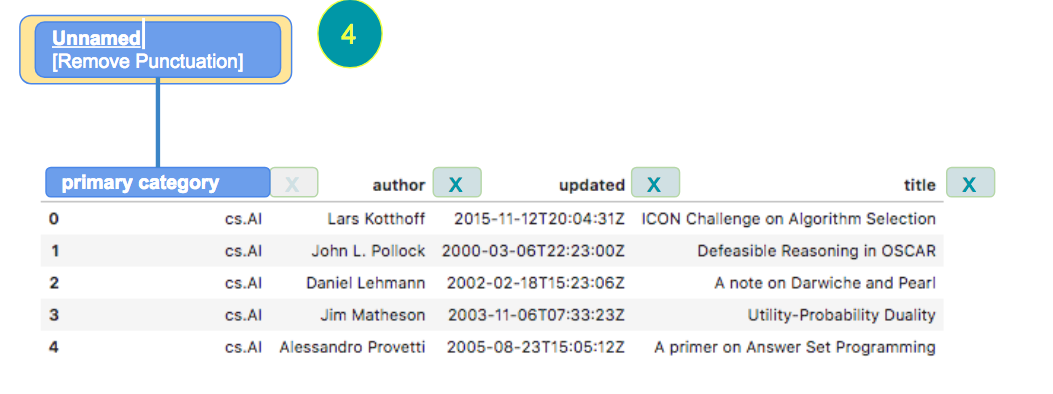
\includegraphics[scale=.3]{figures/m3/wireframe-screen3.png}
\caption{Screen 3: A new block appears that is connected to the selected variable with a cursor prompt to name a new variable}
\label{fig::4}
\end{figure}

    \item Figure~\ref{fig::5} shows a possible view of the outcome of multiple transformations. The information is presented on one screen that given user feedback on the actions taken so far.

\begin{figure}[h]
\centering
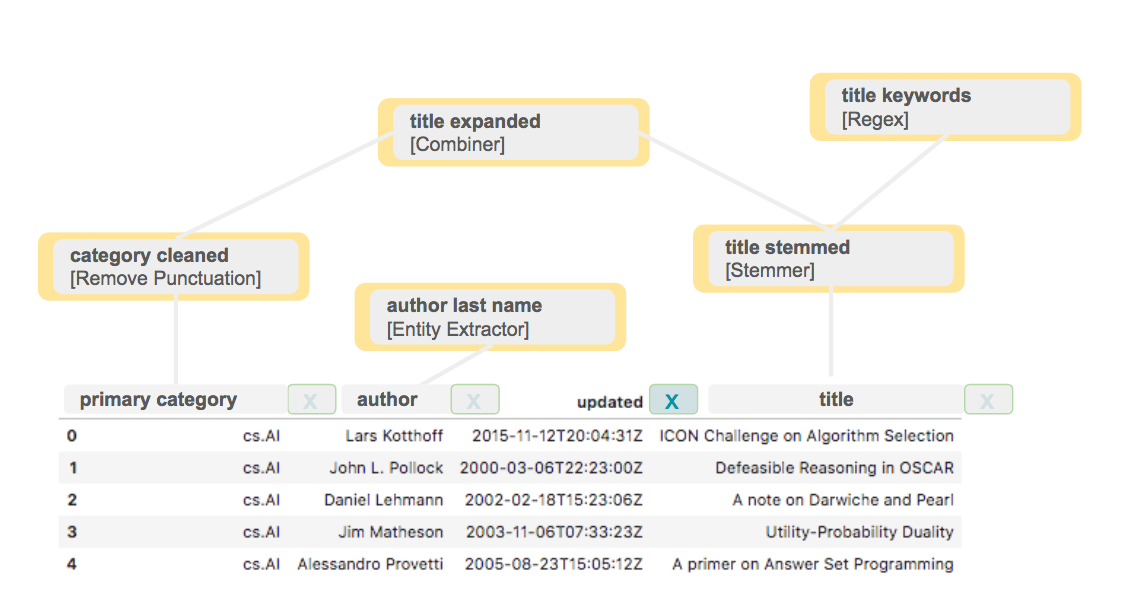
\includegraphics[scale=.3]{figures/m3/wireframe-screen5.png}
\caption{Screen 4: A hypothetical view of the Directed Acyclical Graph (DAG) that is a results of user creating multiple transformations}
\label{fig::5}
\end{figure}

\end{itemize}

\end{document}
